\section{Ideate}
In diesem Abschnitt werden verschiedene Vorgehensweisen im Ideate Schritt des Design Thinking Prozesses aufgezeigt. 

\subsection{Prototyping}
Nachdem wir die ersten Interviews geführt hatten, hatten wir einen ersten Papierprototypen erstellt, damit wir von den Benutzern schnell ein erstes Feedback einholen konnten. Dabei wurde versucht, die durch das Interview ermittelten Hauptfunktionalitäten in ein erstes Design zu überführen. Fürs Prototyping wurde FluidUI verwendet. Mit diesem Prototyping Framework können klickbare (clickable) Prototypen erstellt werden und direkt auf dem mobilen Endgerät getestet werden, sodass der Benutzer schon früh ein Gefühl für die Funktionalitäten und das Design bekommt. Dies stellt sicher, dass Feedback schnell eingeholt und umgesetzt werden kann.


\subsection{Bounded Context mit Eventstorming}
Ein Bounded Context ist ein Pattern im Domain-Driven Design. Martin Fowler beschreibt in seinem Webartikel, dass das Pattern für grosse Teams und Modelle geeignet ist. \cite{fowler2014bound} Mit dem Bounded Context sollte man besser kommunizieren können und die Zuständigkeiten sind klarer definiert und visuell dargestellt. Anhand der Stories und Eventstorming wurden die Bounded Contexte erstellt.

In der unten dargestellten Grafik sind die Kontexte dargestellt. Jeder Kontext hat eine eigene Farbe.

Bounded Contexte:

Kunde:
Der Kunde tritt mit dem ganzen Gamechanger-System in Kontakt, sobald er vom Gamechanger erfährt. Im Zusammenhang mit dem Kunden sind z.B. Marketing, Design, Finanzierung, Sprache/Texte zu betrachtet. Der Kunde kann z.B. als Interessent auftreten, als Nutzer oder auch in anderen Rollen.

Organisation mit Chat, Einladungen, Freunde:
Dieser Context beinhaltet alle wichtigen Aktivitäten, die die Hauptfunktionalität von Gamechanger ausmacht. Chat, Einladungen und Freunde(verwaltung) müssen in diesem Context umbedingt zusammen diskutiert werden und z.B. bei der Technologieauswahl (Kompatibilität) berücksichtig werden.

Identität:
Hier fällt die ganze Verwaltung der Daten, die der Kunde der App überlässt, hinein. Fragestellungen zur Datenbank, Datenschutz, der Registration (onboarding) etc.

Google mit Kalender, Authentifizierung:
Google als grosser Provider gewisser Dienstleistungen ist ein eigener Context, denn viele Services, die verwendet werden, stammen von Google. In diesem Context kümmert man sich um die Anbindung der Services und stellt sich Fragen, wie die externen Services in das System integriert werden können.

Gamification:
Dieser Kontext kümmert sich um alle Angelegenheiten, die die Gamifikation betreffen. Man stellt sich die Frage, wie die Nutzer mehr Freude und Motivation erhalten, den Gamechanger zu nutzen. Dabei kann ein Belohnungssystem in Form von Trophäen helfen und das ganze etwas lebendiger machen. 

\begin{figure}[H]
    \centering
    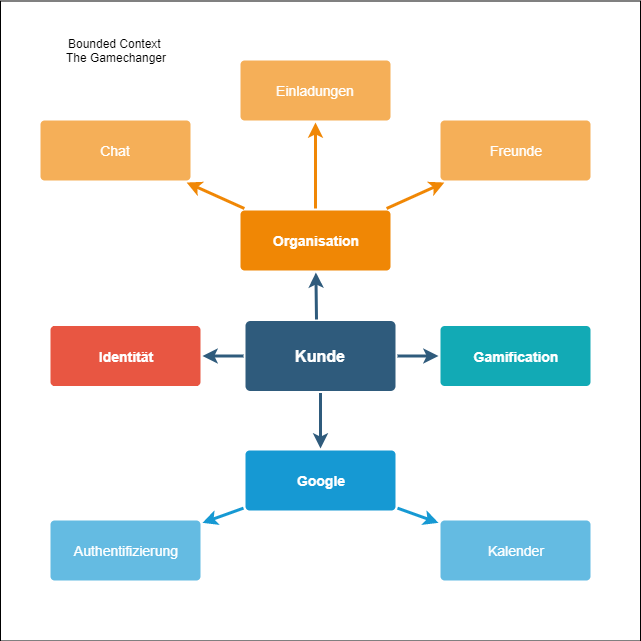
\includegraphics[width=\textwidth]{images/boundedcontext.png}
    \caption{Bounded Context The Gamechanger}
    \label{fig:boundedcontext}
\end{figure}

\subsubsection{Event Storming}
Event Storming ist eine, von Alberto Brandolini, erfundene Methode, bei der man in einem Workshop die Domänen einer Software in kürzester Zeit herausfinden kann. Dabei schreibt man die Domänen einer Software auf orange Post-it's und klebt sie an eine Wand. Danach werden diese mit Kommandos erweitert, die diese Domain-Events auslösen. Die Kommandos werden auf blaue Post-it's links daneben gehängt. Anschliessend werden die Aktoren, die die Kommandos ausführen bestimmt. Danach sollen mögliche Probleme der jeweiligen Domänen auf rote Post-it's geschrieben werden und dazugehängt werden. Zuletzt werden die Domains zu Gruppen aggregiert und diese Aggregationen jeweils auf gelben Post-it's über den Domänen aufgehängt. Das oberste Ziel des Event Storming ist, dass Software Entwickler und Domänenexperten zusammenkommen und voneinander lerne können und dies auf eine spassvolle Art.

Mit Event Storming ist der Prozess der Registrierung analysiert und designt worden. Das Resultat wird in Abbildung \ref{fig:event_storming_registrierung} gezeigt. Die Domain Events beinhalten das Installieren der App, das Öffnen der App und das Anmelden über Google. In einem späteren Increment wird noch die Möglichkeit der Registrierung per E-Mail hinzukommen. Die möglichen Probleme dafür beinhalten Installationsprobleme, Probleme beim Öffnen der App oder bei der Anmeldung.

\begin{figure}[htpb]
    \centering
    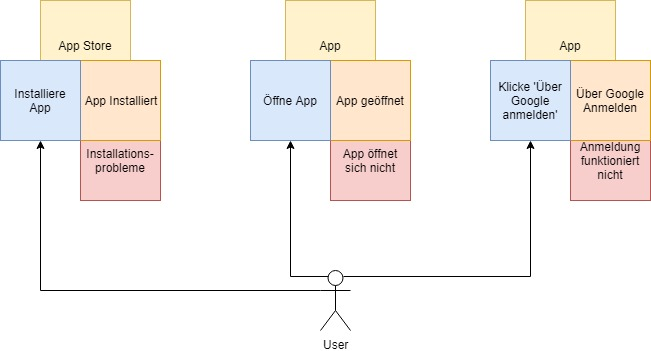
\includegraphics[width=\textwidth]{images/Event_Storming_Registrieren.jpg}
    \caption{Registrierungsprozess mittels Event Storming}
    \label{fig:event_storming_registrierung}
\end{figure}

\subsection{Design}
In diesem Abschnitt werden die Designideen für die Prototypen erläutert. Zuerst wird anhand der Methode Event Storming eine Bounded Context - Map ausgearbeitet. Der Prozess der Authentifizierung wird noch genauer angeschaut und dokumentiert. Danach wird die Navigation und das visuelle Design beschrieben und eine Begründung dargelegt, weshalb genau dieses Design gewählt werden soll.

\subsubsection{Navigation}
Für die Navigation innerhalb der App wurde eine Tabnavigation gewählt. Diese Navigationsart ist sehr verbreitet, da sie alle wichtigen erreichbaren Screens permanent am unteren Ende des Bildschirms anzeigt, sodass der Benutzer zu jeder Zeit die Screens wechseln kann, ohne dabei zuerst über einen Burgerbutton ein Navigationsmenü öffnen muss. Ein weiterer Vorteil dabei ist, dass diese Art der Navigation schon bei vielen bekannten Apps angewendet wird. Der Benutzer kennt diese Art der Navigation schon und kann die Applikation ohne grosse Lernphase direkt bedienen. Beispiele der Tabnavigation bekannter Applikationen sind zum Beispiel die Instagram App oder die LinkedIn App.

\begin{figure}[H]
  \begin{minipage}[b]{0.4\textwidth}
    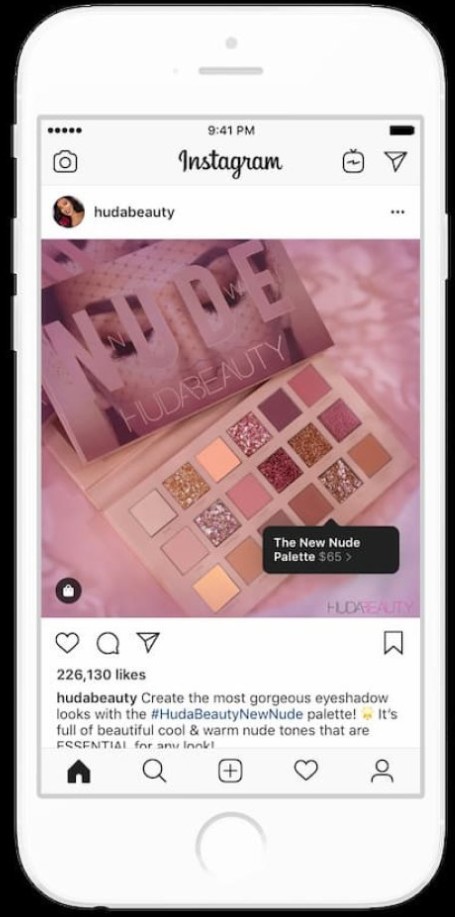
\includegraphics[width=\textwidth]{images/insta.PNG}
    \caption{Instagram Tabnavigation}
    \label{fig:insta}
  \end{minipage}
  \hfill
  \begin{minipage}[b]{0.4\textwidth}
    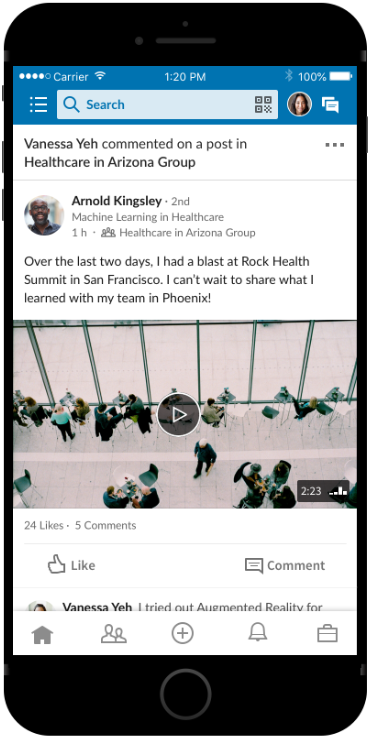
\includegraphics[width=\textwidth]{images/linkedin.PNG}
    \caption{LinkedIn Tabnavigation}
    \label{fig:linkedin}
  \end{minipage}
\end{figure}


\subsubsection{Visuelles Design}
Auch das visuelle Design der Applikation ist wichtig für die Userakzeptanz der App. Da es einerseits sehr viel Zeit beansprucht ein visuelles Design von Grund auf zu konzipieren und da sich die Benutzer andererseits bei neuen Designs zum Teil schwer tun, sich zurecht zu finden, sind wir zum Entschluss gekommen, das \textbf{Material Design} von Google zu verwenden. 

Dieses Design wird von allen Google Services verwendet und das hat den Vorteil, dass sich der Benutzer sehr schnell in der Applikation zurechtfinden kann und sich schon ab der ersten Nutzung zu Hause fühlt. hier abgebildet sind zwei Beispiele für Material Design Komponenten: Ein Button und ein Kalender.

\begin{figure}[H]
  \begin{minipage}[b]{0.4\textwidth}
    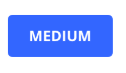
\includegraphics[width=\textwidth]{images/matButton.PNG}
    \caption{Material Design Button}
    \label{fig:matButtom}
  \end{minipage}
  \hfill
  \begin{minipage}[b]{0.4\textwidth}
    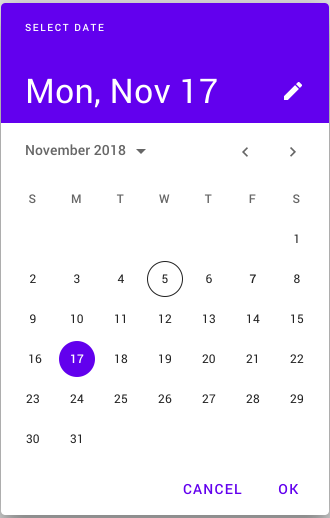
\includegraphics[width=\textwidth]{images/matCalendar.PNG}
    \caption{Material Design Kalender}
    \label{fig:matCalendar}
  \end{minipage}
\end{figure}

Es gibt verschiedenste Frameworks, welche dieses Design unterstützen. Dies erleichtert uns die Arbeit enorm, da wird die einzelnen Komponenten nicht selber designen müssen.

\newpage

\subsection{Erstes Inkrement}
In einem ersten Inkrement wurde versucht, die Hauptfunktionalitäten mit einem intuitiven Design zu erstellen. Das Ziel dabei ist es, dem Benutzer schon ganz am Anfang des Design Prozesses einen ersten Prototypen zeigen zu können, um potentielle Missverständnisse der ersten Interviewrunde aufzudecken und in einer weiteren Iteration zu beheben. Unten abgebildet sind zwei Screens. Der erste Screen ist der Hauptscreen, in welchem die Spielesessions aufgelistet sind. Der ganze Screen ist in drei Bereiche unterteilt, um eine bessere Übersicht über die zukünftigen und abgeschlossenen Sessions und offenen Einladungen zu erhalten. 

\begin{figure}[H]
  \begin{minipage}[b]{0.4\textwidth}
    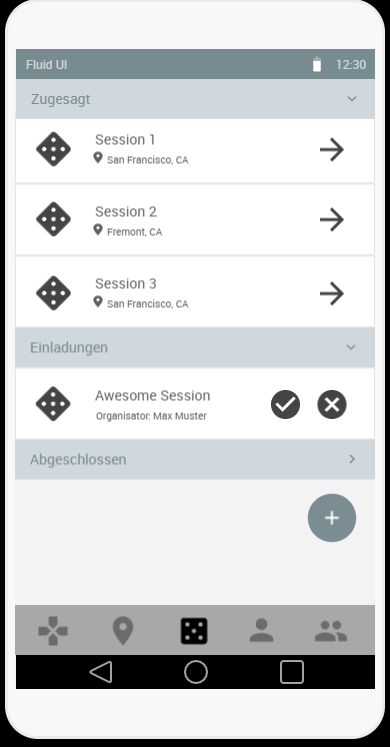
\includegraphics[width=\textwidth]{images/MainScreen.PNG}
    \caption{Haupt Screen}
    \label{fig:mainScreen}
  \end{minipage}
  \hfill
  \begin{minipage}[b]{0.4\textwidth}
    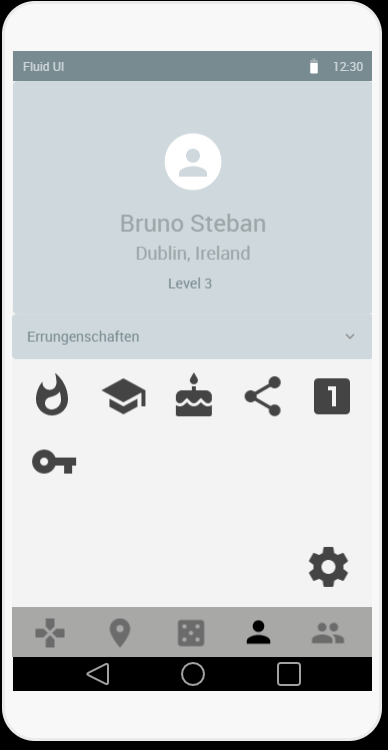
\includegraphics[width=\textwidth]{images/ProfileScreen.PNG}
    \caption{Profil Screen}
    \label{fig:profileScreen}
  \end{minipage}
\end{figure}

Die Navigationsleiste am unteren Ende des Screens beinhaltet fünf Tabs: Ganz links ist der Tab für offene Quests, welche der Spieler erfüllen kann um Errungenschaften zu erhalten. Darauffolgend ist der Map Tab, welcher eine Karte der physikalischen Umgebung des Spielers und öffentliche Sessions anzeigt, bei welchen sich der Spieler anmelden kann. In der Mitte der Navigationsleiste befindet sich die Hauptseite, in denen die Sessions angezeigt werden und wo der Spieler auch eine neue Session erstellen kann. Der zweite Tab von rechts beinhaltet den Profil-Screen, welcher Informationen zum Spieler und allgemeine Einstellungen der Applikation anzeigt. Der letzte Tab zeigt den Social-Screen, indem Freunde des Benutzers und seine Spielgruppen angezeigt und verwaltet werden können.
\newline
Bei der Navigationsleiste ist es wichtig, dass nicht mehr als fünf Tabs vorhanden sind, da diese Navigationsart sonst schnell unübersichtlich wird. Die meisten Apps mit einer Tabnavigation benutzen fünf Tabs (wie zum Beispiel die Instagram und LinkedIn App von oben), da sich dadurch eine gute Trennung der Funktionalitäten ergibt und die einzelnen Tabs nicht zu viele Inhalte besitzen.

Das Design mit den zuklappbaren Listen erstreckt sich über alle Screens. Damit hat der Spieler immer alle wichtigen Daten zur Hand und kann nicht benötigte Informationen rasch und einfach ausblenden. Ein weiteres wiederkehrendens Material Design Element ist der \textbf{+} Button. Dieser wird überall als Button zum Erzeugen einer neuen Entität erkannt. Wenn der Benutzer also den Plus Button im Social Screen bei der Freundesliste sieht, ist ihm sofort klar, dass man mit diesem Button einen neuen Freund hinzufügen kann. Solche wiederkehrenden Bedienelemente erleichtern es dem Benutzer enorm, sich in der App zurecht zu finden und er kann die Interaktionssabläufe schnell erlernen.

Unten sind zwei weitere Screens abgebildet: Der linke Screen zeigt das Layout wenn ein Benutzer eine neue Session erstellen will. Auch hier ist wieder der Plus Button ersichtlich, um neue Daten hinzuzufügen sowie auch Spieler oder ganze Spielgruppen einzuladen (auf dem Screen nicht ersichtlich, da der User scrollen müsste um diese Gruppeneinladungen zu tätigen). Der rechte Screen gibt einen Überblick úber die sozialen Kontakte sowie die festen Spielgruppen, in der sich der Benutzer befindet.

\begin{figure}[H]
  \begin{minipage}[b]{0.4\textwidth}
    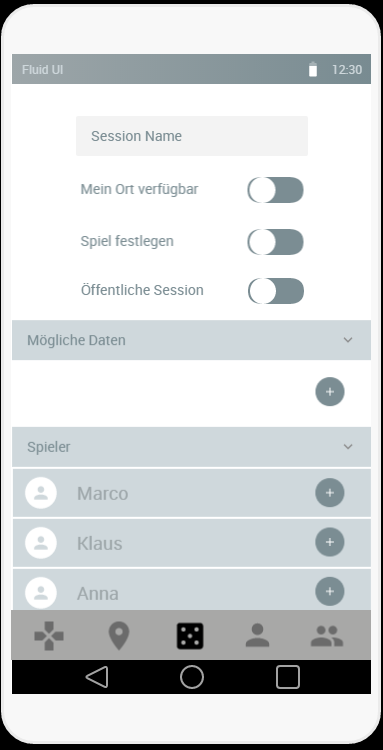
\includegraphics[width=\textwidth]{images/newSession.PNG}
    \caption{Haupt Screen}
    \label{fig:newSession}
  \end{minipage}
  \hfill
  \begin{minipage}[b]{0.4\textwidth}
    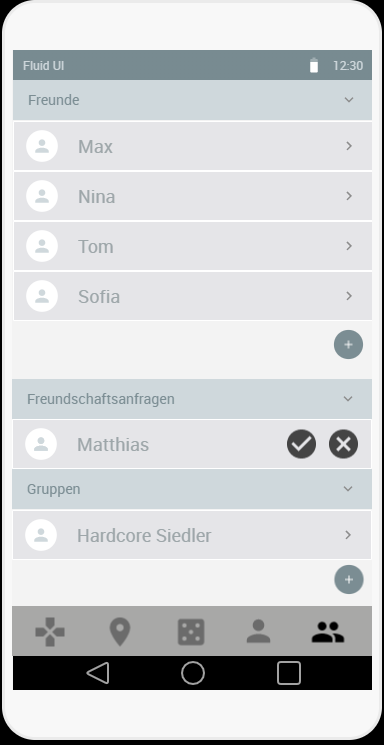
\includegraphics[width=\textwidth]{images/FreundundGruppenScreen.PNG}
    \caption{Profil Screen}
    \label{fig:SocialScreen}
  \end{minipage}
\end{figure}

Der nächste Schritt ist es nun, dem Benutzer (Samuel Müller) diesen Prototypen zu zeigen und Test-Aufgaben zu definieren, welche der Benutzer mit dem Prototypen erledigen muss, um festzustellen, welche Navigations- und Interaktionsabläufe Verwirrung stiften. Das resultierende Feedback kann dann in der nächsten Iteration des Prototypings umgesetzt werden.

\subsection{Implementation erster Komponenten}
Als erste Komponenten haben wir den Authentisierungs-Screen und den Haupt-Screen implementiert. Für den Anfang haben wir uns entschieden, die Authentisierung mit einem schon vorhandenen Google Account über OAuth durchzuführen. Die Anbindung weiterer OAuth Anbieter wie zum Beispiel Facebook, Twitter oder GitHub kann dann zu einem späteren Zeitpunkt ähnlich wie das Google OAuth erfolgen. 
\newline
Das Ziel der Implementation dieser ersten beiden Komponenten ist es, zu zeigen, dass die gewählten Technologien miteinander funktionieren und das Projekt so durchgeführt werden kann. Es wurde der Authentisierungs-Screen und der Haupt-Screen gewählt, da diese sehr nahe miteinander verknüpft sind, sprich nach der Authentisierung kommt der User direkt auf den Haupt-Screen. Da diese beiden Komponenten auch die ersten Berührungspunkte des Users mit der App sind, macht es unserer Meinung nach Sinn, dieser zu erst zu implementieren.

\subsubsection{Konzeption des GUI}
Eine erste Konzeption des GUI wurde schon beim Prototyping durchgeführt. Hier nochmals die geplanten GUI Komponenten:

\begin{figure}[H]
  \begin{minipage}[b]{0.4\textwidth}
    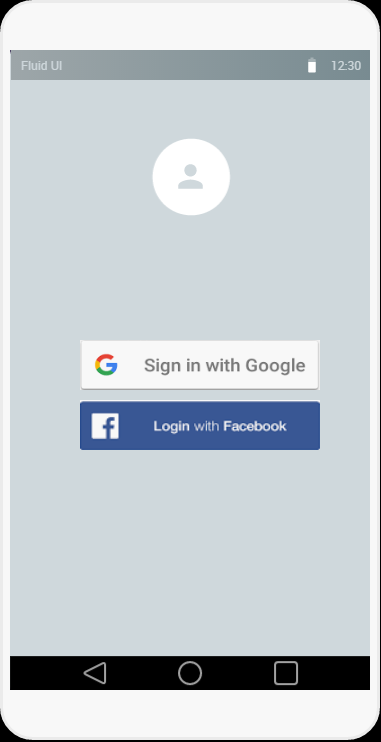
\includegraphics[width=\textwidth]{images/loginscreen_prototyp.PNG}
    \caption{Authentisierungs-Screen}
    \label{fig:loginscreen_2}
  \end{minipage}
  \hfill
  \begin{minipage}[b]{0.4\textwidth}
    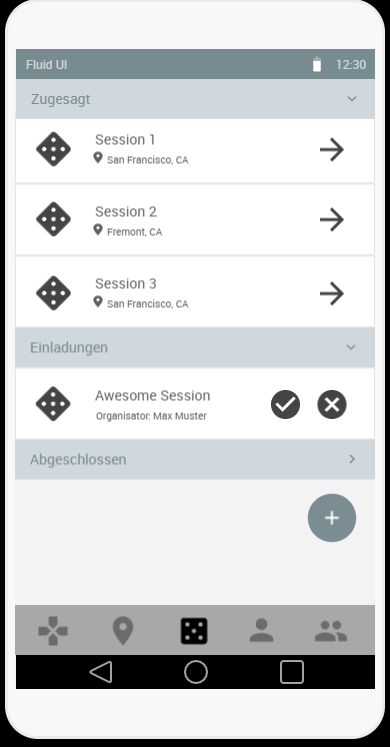
\includegraphics[width=\textwidth]{images/MainScreen.PNG}
    \caption{Haupt-Screen}
    \label{fig:mainschreen_2}
  \end{minipage}
\end{figure}

\subsubsection{Implementation des GUI}
Bei der Implementation des GUI haben wir uns am Prototypen orientiert. Wie oben erwähnt, haben wir als erstes die Authentisierung mit OAuth über das Google Konto des Users implementiert. Folgend ist der Authentisierungsprozess mit Screenshots der Applikation abgebildet:

\begin{figure}[H]
  \begin{minipage}[b]{0.4\textwidth}
    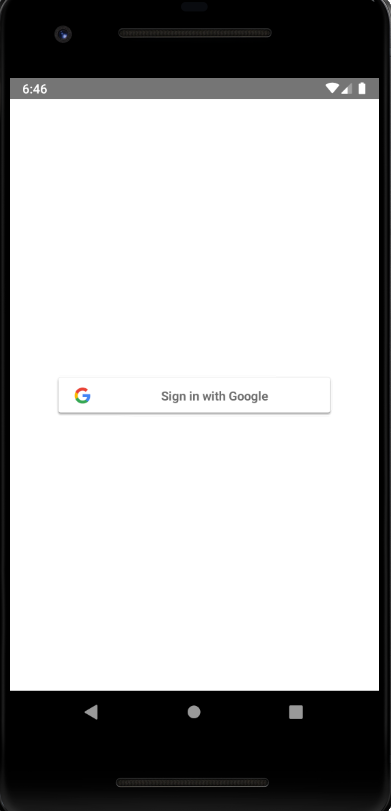
\includegraphics[width=\textwidth]{images/signinwithgoogle_implementation1.PNG}
    \caption{Authentisierungs-Screen Implementation}
    \label{fig:loginscreen_3}
  \end{minipage}
  \hfill
  \begin{minipage}[b]{0.4\textwidth}
    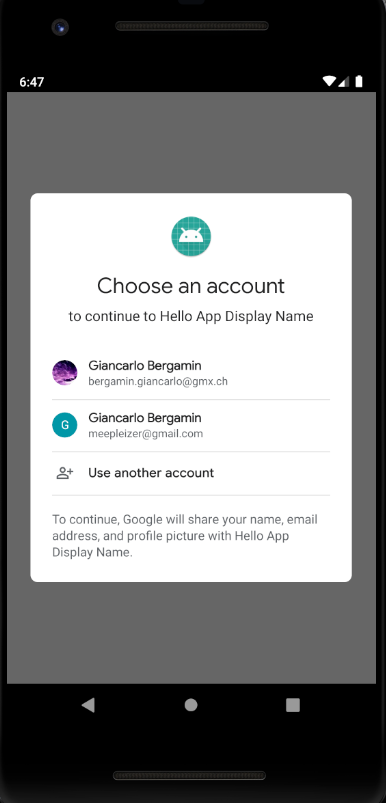
\includegraphics[width=\textwidth]{images/signinwithgoogle_implementation2.PNG}
    \caption{PopUp OAuth Google}
    \label{fig:oauth}
  \end{minipage}
\end{figure}

Nachdem man das Konto ausgewählt hat, mit dem man sich einloggen möchte, wird man direkt auf den Haupt-Screen weitergeleitet. Unten sind zwei Haupt-Screens der zwei verschiedenen Testuser dargestellt. Die Abbildung zeigt, dass userspezifische Daten geladen worden sind, nämlich die geplanten Sessions der User.

\begin{figure}[H]
  \begin{minipage}[b]{0.4\textwidth}
    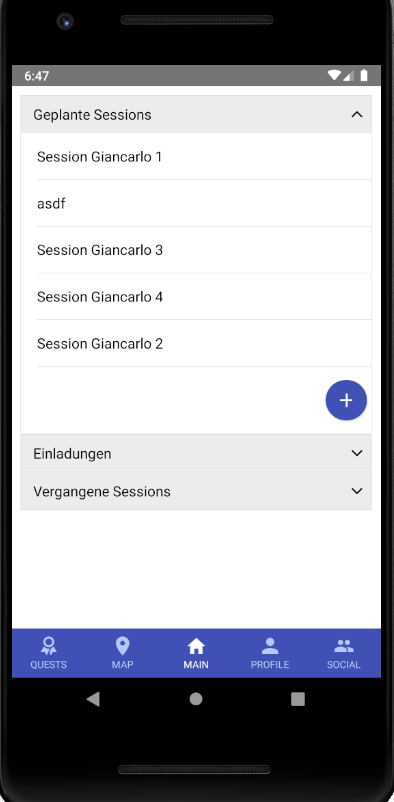
\includegraphics[width=\textwidth]{images/mainscreen_implementation1.PNG}
    \caption{Main-Screen Implementation User A}
    \label{fig:mainscreenusera}
  \end{minipage}
  \hfill
  \begin{minipage}[b]{0.4\textwidth}
    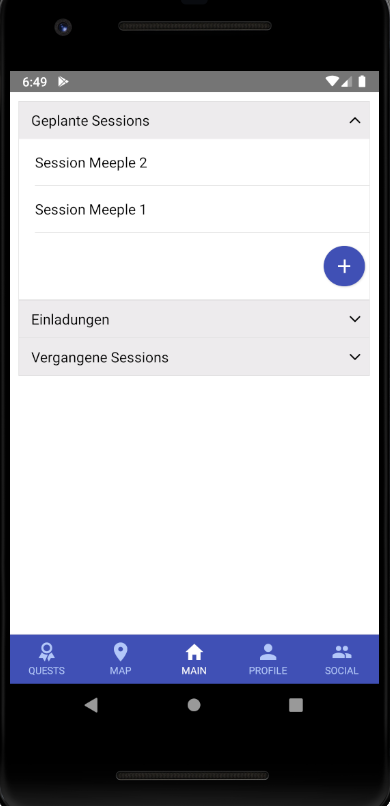
\includegraphics[width=\textwidth]{images/mainscreen_implementation_meeple.PNG}
    \caption{Main-Screen Implementation User B}
    \label{fig:mainscreenuserb}
  \end{minipage}
\end{figure}

Wie man sieht, haben wir die drei aufklappbaren Listen, wie im Prototyp konzipiert, implementiert. Die Implementation der Einladungen und der Vergangenen Sessions haben wir noch nicht fertiggestellt. Diese können jedoch analog zu den geplanten Sessions implementiert werden. Auch die Tabnavigation wurde schon implementiert.

\subsubsection{Testing und Deployment}
Der erstellte Code wurde danach mit git auf das remote Repository gepushed und dies triggered dann das Testing und das Deployment direkt auf die Mobilgeräte der Betauser (siehe Abschnitt CI/CD).